% THIS IS AN EXAMPLE DOCUMENT FOR VLDB 2012
% based on ACM SIGPROC-SP.TEX VERSION 2.7
% Modified by  Gerald Weber <gerald@cs.auckland.ac.nz>
% Removed the requirement to include *bbl file in here. (AhmetSacan, Sep2012)
% Fixed the equation on page 3 to prevent line overflow. (AhmetSacan, Sep2012)

\documentclass{vldb}
\usepackage{graphicx}
\usepackage{balance}  % for  \balance command ON LAST PAGE  (only there!)
\usepackage{fontspec}
\usepackage{hyperref}
\graphicspath{{figures/}}
\usepackage{enumitem}

\begin{document}

% ****************** TITLE ****************************************

\title{The RADStack: Open Source Lambda Architecture for Interactive Analytics}

% possible, but not really needed or used for PVLDB:
%\subtitle{[Extended Abstract]
%\titlenote{A full version of this paper is available as\textit{Author's Guide to Preparing ACM SIG Proceedings Using \LaTeX$2_\epsilon$\ and BibTeX} at \texttt{www.acm.org/eaddress.htm}}}

% ****************** AUTHORS **************************************

% You need the command \numberofauthors to handle the 'placement
% and alignment' of the authors beneath the title.
%
% For aesthetic reasons, we recommend 'three authors at a time'
% i.e. three 'name/affiliation blocks' be placed beneath the title.
%
% NOTE: You are NOT restricted in how many 'rows' of
% "name/affiliations" may appear. We just ask that you restrict
% the number of 'columns' to three.
%
% Because of the available 'opening page real-estate'
% we ask you to refrain from putting more than six authors
% (two rows with three columns) beneath the article title.
% More than six makes the first-page appear very cluttered indeed.
%
% Use the \alignauthor commands to handle the names
% and affiliations for an 'aesthetic maximum' of six authors.
% Add names, affiliations, addresses for
% the seventh etc. author(s) as the argument for the
% \additionalauthors command.
% These 'additional authors' will be output/set for you
% without further effort on your part as the last section in
% the body of your article BEFORE References or any Appendices.

\numberofauthors{6} %  in this sample file, there are a *total*
% of EIGHT authors. SIX appear on the 'first-page' (for formatting
% reasons) and the remaining two appear in the \additionalauthors section.

\author{
% You can go ahead and credit any number of authors here,
% e.g. one 'row of three' or two rows (consisting of one row of three
% and a second row of one, two or three).
%
% The command \alignauthor (no curly braces needed) should
% precede each author name, affiliation/snail-mail address and
% e-mail address. Additionally, tag each line of
% affiliation/address with \affaddr, and tag the
% e-mail address with \email.
%
% 1st. author
\alignauthor
Fangjin Yang\\
       \email{fangjinyang@gmail.com}
% 2nd. author
\alignauthor
Gian Merlino\\
       \email{gianmerlino@gmail.com}
% 3rd. author
\alignauthor 
Xavier Léauté\\
       \affaddr{Metamarkets Group, Inc.}\\
       \email{xavier@metamarkets.com}
\and  % use '\and' if you need 'another row' of author names
% 4th. author
\alignauthor
Nishant Bangarwa\\
       \affaddr{Metamarkets Group, Inc.}\\
       \email{nishant.bangarwa@metamarkets.com}
% 5th. author
\alignauthor
Charles Allen\\
       \affaddr{Metamarkets Group, Inc.}\\
       \email{charles.allen@metamarkets.com}
% 6th. author
\alignauthor
Eric Tschetter\\
       \email{echeddar@gmail.com}
}
% There's nothing stopping you putting the seventh, eighth, etc.
% author on the opening page (as the 'third row') but we ask,
% for aesthetic reasons that you place these 'additional authors'
% in the \additional authors block, viz.
% Just remember to make sure that the TOTAL number of authors
% is the number that will appear on the first page PLUS the
% number that will appear in the \additionalauthors section.

\maketitle

\begin{abstract}
The Real-time Analytics Data Stack, colloquially referred to
as the RADStack, is an open-source data analytics stack designed to provide
fast, flexible queries over up-to-the-second data. It is designed to overcome
the limitations of either a purely batch processing system (which takes too
long to surface new events) or a purely real-time system (which is difficult to
ensure that no data is left behind and there is often no way to correct data
after initial processing). It will seamlessly return best-effort results on
very recent data combined with guaranteed-correct results on older data. In
this paper, we introduce the architecture of the RADStack and discuss our
methods of providing interactive analytics and a flexible data processing
environment to handle a variety of real-world workloads.
\end{abstract}

\section{Introduction}
The rapid growth of the Hadoop\cite{shvachko2010hadoop} ecosystem has enabled
many organizations to flexibly process and gain insights from large quantities
of data. These insights are typically business intelligence questions, or
OnLine Analytical Processing (OLAP) queries. Hadoop has proven to be an
extremely effective framework capable of providing many analytical insights and
is able to solve a wide range of distributed computing problems. However, as
much as Hadoop is lauded for its wide range of use cases, it is derided for its
high latency in processing and returning results. A common approach to surface
data insights is to run MapReduce jobs that may take several hours to complete.
 
Data analysis and data-driven applications are becoming increasingly important
in industry, and the long query times seen with using frameworks such as Hadoop
are becoming increasingly intolerable. User facing applications are replacing
traditional reporting interfaces as the preferred means for organizations to
derive value from their datasets. In order to provide an interactive user
experience, user interactions with data-driven applications must complete in an
order of milliseconds. Because most of these interactions revolve around data
exploration and computation, organizations quickly realized that in order
support low latency queries, dedicated serving layers are necessary. Today,
most of these serving layers are Relational Database Management Systems (RDBMS)
or NoSQL key/value stores. Neither RDBMS nor NoSQL key/value stores are
particularly designed for analytics, but these technologies are still
frequently selected as serving layers because of their general popularity.
Hence, solutions that involve these technologies can be inflexible, or suffer
from architecture drawbacks that prevent them from returning queries fast
enough to power interactive, user-facing applications \cite{tschetter2011druid}.

An ideal serving layer by itself is still insufficient as a complete analytics
solution. In most real-world use cases, raw data cannot be directly stored in
the serving layer. Raw data suffers from many imperfections and must first be
processed (transformed, or cleaned) before it is usable. Hadoop remains a
popular option to process raw data and many organizations first process raw
data in Hadoop before loading the result into the serving layer. The drawback
of this approach is that loading and processing batch data is slow, and
insights on events are often obtained hours after the events have occurred [].
 
To address the problem of delays in data freshness caused by batch processing
frameworks, numerous open-source stream processing frameworks such as Apache
Storm\cite{marz2013storm}, Apache Spark Streaming\cite{zaharia2012discretized},
and Apache Samza\cite{2014samza} have been gaining popularity for offering a
low-latency model to ingest and process event streams. These stream processing
frameworks have enabled data processing at near real-time speeds. The drawback
of popular open-source stream processors is that they do not necessarily
provide the same correctness guarantees as batch processing frameworks. Events
can come in days late, and may need to be corrected after the fact. Large
blocks of data may also need to be reprocessed at any time as new columns are
added or removed.
 
The RADStack is an open source, end-to-end solution meant to offer flexible,
low-latency analytic queries on near real-time data. The solution combines the
low latency guarantees of stream processors and the correctness and flexibility
guarantees of batch processors. It also introduces a serving layer specifically
designed for interactive analytics. The stack’s main building blocks are Apache
Kafka\cite{kreps2011kafka}, Apache Samza, Apache Hadoop, and Druid[], and we’ve
found that the combination of technologies is flexible enough to handle a wide
variety of processing requirements and query loads. Each piece of the stack is
designed to do a specific set of things very well. This paper will cover the
details and design principles of the RADStack. Our contributions are around the
architecture of the stack itself, the introduction of Druid as a serving layer,
and our model for unifying real-time and historical workflows.
 
The structure of the paper is as follows: Section \ref{sec:background}
describes the problems and use cases that led to the creation of the RADStack.
Section \ref{sec:serving} describes Druid, the serving layer of the stack, and
how Druid is built for real-time and batch data ingestion, as well as
exploratory analytics. Section \ref{sec:processing} covers the role of Samza
and Hadoop for data processing, and Section \ref{sec:delivery} describes the
role of Kafka for event delivery. In Section \ref{sec:performance}, we present
our production metrics.  Section \ref{sec:experiences} presents our experiences
with running the RADStack in production, and in Section \ref{sec:related} we
discuss the related work.

\section{Background}
\label{sec:background}

\begin{table*}
  \centering
  \begin{tabular}{| l | l | l | l | l | l | l | l |}
    \hline
    \textbf{Timestamp} & \textbf{Publisher} & \textbf{Advertiser} & \textbf{Gender} & \textbf{City} & \textbf{Click} & \textbf{Price} \\ \hline
    2011-01-01T01:01:35Z & bieberfever.com & google.com & Male & San Francisco & 0 & 0.65 \\ \hline
    2011-01-01T01:03:63Z & bieberfever.com & google.com & Male & Waterloo & 0 & 0.62 \\ \hline
    2011-01-01T01:04:51Z & bieberfever.com & google.com & Male & Calgary & 1 & 0.45 \\ \hline
    2011-01-01T01:00:00Z & ultratrimfast.com & google.com & Female & Taiyuan & 0 & 0.87 \\ \hline
    2011-01-01T02:00:00Z & ultratrimfast.com & google.com & Female & New York & 0 & 0.99 \\ \hline
    2011-01-01T02:00:00Z & ultratrimfast.com & google.com & Female & Vancouver & 1 & 1.53 \\ \hline
  \end{tabular}
  \caption{Sample ad data. These events are created when users view or click on ads.}
  \label{tab:sample_data}
\end{table*}

The development of RADStack came about iteratively. Different technologies were
introduced to address various problems and use cases that came up over time.
The initial concept of the RADStack started at Metamarkets, an analytics
startup focused in the advertising technology space, and has since been adopted
by other technology companies \cite{2014yahoo}. In the early days of Metamarkets, we wanted
to build an analytics dashboard where users could arbitrarily explore their
data. An example of the data found in online advertising space is shown in
Table~\ref{tab:sample_data}. An example dashboard is shown in Figure [].
 
The data shown in Table~\ref{tab:sample_data} is fairly standard in OLAP
workflows. The data is transactional (timeseries data) and tends to be very
append heavy. Each event is comprised of three components: a timestamp
indicating when the event occurred; a set of dimensions indicating various
attributes about the event; and a set of metrics concerning the event. Our goal
is to rapidly compute drill-down and aggregates with this data, to answer
questions such as “How many clicks occurred over the span of one week for
publisher google.com?” or “How many impressions were seen over the last quarter
from the city of San Francisco?” We wanted to issue queries over any arbitrary
number of dimensions and have results return in at most several hundred
milliseconds.
 
In addition to the query latency needs, we needed to support multi-tenancy.
User-facing applications often face highly concurrent workloads and good
applications need to provide relatively consistent performance to all users.
Finally, we needed our backend infrastructure to be highly available. Downtime
is costly and many businesses cannot afford to wait if a system is unavailable
in the face of software upgrades or network failure. Downtime for startups, who
often lack proper internal operations management, can determine business
success or failure.
 
Following industry standard practices, we evaluated various options for a
serving layer. We tried to select a serving layer that was optimized for the
types of queries we wanted to make, and we initially began our experiments with
PostgreSQL\cite{stonebraker1987extendability}. Our setup with PostgreSQL
followed the common conventions of using RDBMSs as data warehouses. We modeled
the advertising data using a star schema, we had a set of aggregate tables to
increase aggregation performance, and we had a query cache to further speed up
queries.

\begin{table*}
  \centering
  \scriptsize\begin{tabular}{| l | l |}
    \hline
    Native Benchmark Scan Rate & \~5.5M rows/second/core \\ \hline
    1 day of summarized aggregates & 60M+ rows \\ \hline
    1 query over 1 week, 16 cores & \~5 seconds \\ \hline
    Page load with 20 queries over a week of data & several minutes \\ \hline
  \end{tabular}
  \normalsize
  \caption{Initial evaluation with PostgreSQL on m2.2xlarge EC2 node.}
  \label{tab:postgres_results}
\end{table*}
 
Our findings with PostgreSQL are shown in Table \ref{tab:postgres_results}.
Query latencies were generally acceptable if the results were cached, less
acceptable if we hit aggregate tables, and unacceptable if we needed to scan
the base fact table. A single page load of the first version of our
application, which issued about 20 concurrent queries to the serving layer and
only required aggregating a few metrics, took several minutes to complete. This
was too slow to power an interactive application. We quickly realized a row
store, and relational model as a whole, was a sub-optimal choice for the
application we were trying to build.

We next evaluated HBase \cite{george2011hbase}, a NoSQL key/value store. As is common with using
key/value stores, we precomputed the total set of queries we anticipated users
would make. An example of this precomputation is shown in Figure []. Our
results with HBase are shown in Table []. Queries were obviously fast as we
were effectively doing O(1) lookups into maps. However, the solution was not
particularly flexible; if something precomputed, it wasn’t queryable, and the
precomputation time became an incredible pain point. We attempted to build
iceberg cubes as described in [], restricting the space of our
pre-computations, but even then the precomputation times were unbearably slow.
Our entire evaluation of both RDBMS and key/value stores is described in detail
in \cite{tschetter2011druid}.

Druid was developed in an attempt to solve some of the problems seen with
traditional serving layers. Druid was designed from the ground up to provide
arbitrary data exploration, low latency aggregations, and fast data ingestion.
Druid was also designed to intake fully denormalized data, and moves away from
the traditional relational model. Since much of raw data is not denormalized,
it must be processed before it can be ingested and queried. Multiple streams of
data had to be joined, cleaned up, and transformed before it was usable in
Druid, but that was the trade-off we decided was necessary in order to get the
performance necessary for an interactive data application. We introduced stream
processing to our stack to provide the business logic processing that was
required before raw data could be loaded into Druid. Our streaming processing
jobs range from simple data transformations, such as id to name lookups, up to
complex operations such as multi-stream joins. Pairing Druid with a stream
processor enabled flexible data processing and querying, but because events
were delivered from many different locations and sources, we also required
technology that was designed for high throughput event delivery. Thus, we added
Kafka to our stack, and Kafka became the event delivery endpoint for our
clients. Kafka provided a highly available message bus. Samza read data from
Kafka, processed it, and delivered the output to Druid. 

Our stack would be complete here if real-time processing were perfect. Sadly,
the open source stream processing space is still young. Processing jobs can go
down for extended periods of time and events may be delivered more than once.
These are realities of any production data pipeline. To overcome these issues,
we included Hadoop in our stack to periodically clean up any data generated by
the real-time pipeline. We stored a copy of the raw events we received in a
distributed file system, and periodically ran batch processing jobs over this
data. The high level architecture of our setup is shown in Figure [], and
illustrates the pieces of the RADStack. Each component in the RADStack is
designed to do a specific set of things well, and there is isolation in terms
of functionality. Individual components can entirely fail without impacting the
services of the other components.

\begin{figure*}
\centering
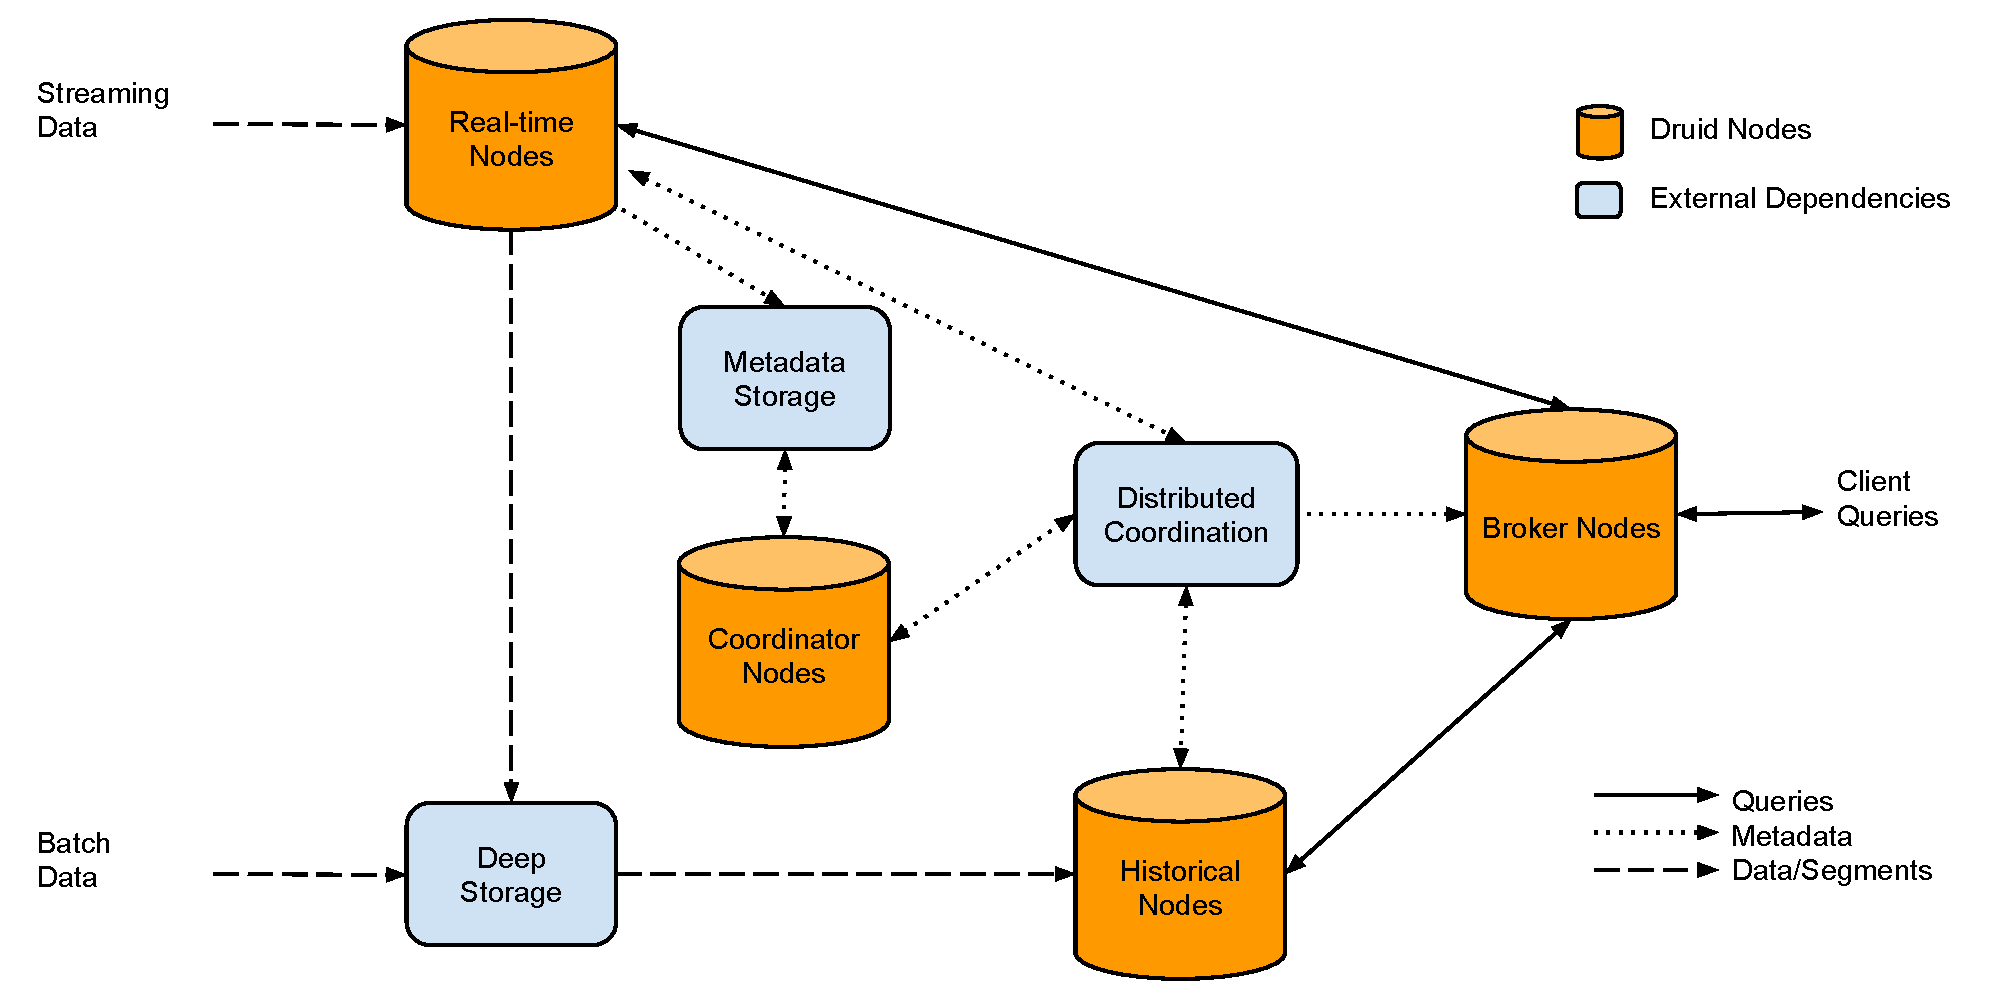
\includegraphics[width = 4.5in]{cluster}
\caption{An overview of a Druid cluster and the flow of data through the cluster.}
\label{fig:cluster}
\end{figure*}

\section{The Serving Layer}
\label{sec:serving}
Druid acts as the serving layer in the RADStack. Druid is a column-oriented
data store designed for exploratory analytics. A Druid cluster consists of
different types of nodes and, similar to the overall design of the RADStack,
each node type is instrumented to perform a specific set of things well. We
believe this design separates concerns and simplifies the complexity of the
overall system. The different node types operate fairly independent of each
other and there is minimal interaction among them. Hence, intra-cluster
communication failures have minimal impact on data availability. To solve
complex data analysis problems, the different node types come together to form
a fully working system. The composition of and flow of data in a Druid cluster
are shown in Figure~\ref{fig:cluster}.

\subsection{Segments}
\label{sec:segments}
Data tables in Druid (called data sources) are collections of timestamped
events and partitioned into a set of segments, where each segment is typically
5–10 million rows. We define a segment as a collection of rows of data that
span some period of time. Segments represent the fundamental storage unit in
Druid and Druid queries only understand how to scan segments. 

Druid always requires a timestamp column as a method of simplifying data
distribution policies, data retention policies, and first level query pruning.
Druid partitions its data sources into well defined time intervals, typically
an hour or a day, and may further partition on values from other columns to
achieve the desired segment size. The time granularity to partition segments is
a function of data volume and time range. A data set with timestamps spread
over a year is better partitioned by day, and a data set with timestamps spread
over a day is better partitioned by hour. 

Segments are uniquely identified by a data source identifier, the time interval
of the data, and a version string that increases whenever a new segment is
created. The version string indicates the freshness of segment data; segments
with later versions have newer views of data (over some time range) than
segments with older versions. This segment metadata is used by the system for
concurrency control; read operations always access data in a particular time
range from the segments with the latest version identifiers for that time
range.

Druid segments are stored in a column orientation. Given that Druid is best
used for aggregating event streams (all data going into Druid must have a
timestamp), the advantages of storing aggregate information as columns rather
than rows are well documented \cite{abadi2008column}. Column storage allows for
more efficient CPU usage as only what is needed is actually loaded and scanned.
In a row oriented data store, all columns associated with a row must be scanned
as part of an aggregation. The additional scan time can introduce significant
performance degradations \cite{abadi2008column}.

Druid nodes use one thread to scan one segment at a time, and the amount of
data that can be scanned in parallel is directly correlated to the number of
available cores in the cluster. Segments are immutable, and immutability
confers a few advantages. Immutable segments enable read consistency, and
multiple threads can scan the same segment at the same. This helps enable
higher read throughput. 

A single query may require scanning thousands of segments concurrently, and
many queries may run at the same time. We want to ensure that the entire
cluster is not starved out while a single expensive query is executing. Thus,
segments have an upper limit in how much data they can hold, and are designed
to be scanned in a few milliseconds. By keeping segment computation very fast,
cores and other resources are constantly being yielded.This ensures segments
from different queries are always being scanned.

Druid segments are very self-contained for the time interval of data that they
hold. Column data is stored directly in the segment. Druid has multiple column
types to represent various data formats. For typical OLAP data, timestamps are
stored in long columns, dimensions are stored in string columns, and measures
(or metrics as they are called in Druid) are stored in int, float, long or
double columns. Depending on the column type, different compression methods may
be used. Metric columns are compressed using LZ4 [] compression. String columns
are dictionary encoded, similar to other data stores such as PowerDrill\cite{hall2012processing}.
Additional indexes may be created for particular columns. For example, Druid
will by default create inverted indexes for string columns.

\subsection{Exploratory Analytics}

Real-world OLAP queries often ask for the aggregated totals for some set of
metrics, filtered for some boolean expressions of dimension specifications,
over some period of time. An example query for Table~\ref{tab:sample_data} may
ask: “How many clicks occurred where publisher is bieberfever.com and users
were male?”. 

Consider the publisher column in Table~\ref{tab:sample_data}, a string column.
For each unique publisher in Table 1, our inverted index tells us in which
table rows a particular page is seen. Our inverted index looks like the
following:

{\small\begin{verbatim}
bieberfever.com   -> rows [0, 1, 2] -> [1][1][1][0][0][0]
ultratrimfast.com -> rows [3, 4, 5] -> [0][0][0][1][1][1]
\end{verbatim}}

In the binary array, the array indices represent our rows, and the array values
indicate whether a particular value was seen. In our example, bieberfever.com
is seen in rows 0, 1 and 2. To know which rows contain bieberfever.com or
ultratrimfast.com, we can OR together the two arrays.

{\small\begin{verbatim}
[1][1][1][0][0][0] OR [0][0][0][1][1][1] = [1][1][1][1][1][1]
\end{verbatim}}

Our query is aggregating two metrics. Our metrics are also stored in a column
orientation such as the following:

{\small\begin{verbatim}
Clicks -> [0, 0, 1, 0, 0, 1]
Price  -> [0.65, 0.62. 0.45, 0.87, 0.99, 1.53]
\end{verbatim}}

We can quickly load up only the metric columns we need for the query. We do not
need to scan the entire metric column for a given query. For example, queries
for results where publisher is bieberfever.com only requires scanning rows 0,
1, and 2 in the metrics column. The inverted indexes tell us exactly the rows
we need to scan, and Druid has an internal cursor to only walk through the rows
that match the final inverted index.

\subsection{Streaming Data Ingestion}
Druid real-time nodes encapsulate the functionality to ingest and query event
streams. Events indexed via these nodes are immediately available for querying.
The nodes are only concerned with events for some small time range and
periodically hand off immutable batches of events they have collected over this
small time range to other nodes in the Druid cluster that are specialized in
dealing with batches of immutable events. The nodes announce their online state
and the data they serve in Zookeeper\cite{hunt2010zookeeper}.

\begin{figure}
\centering
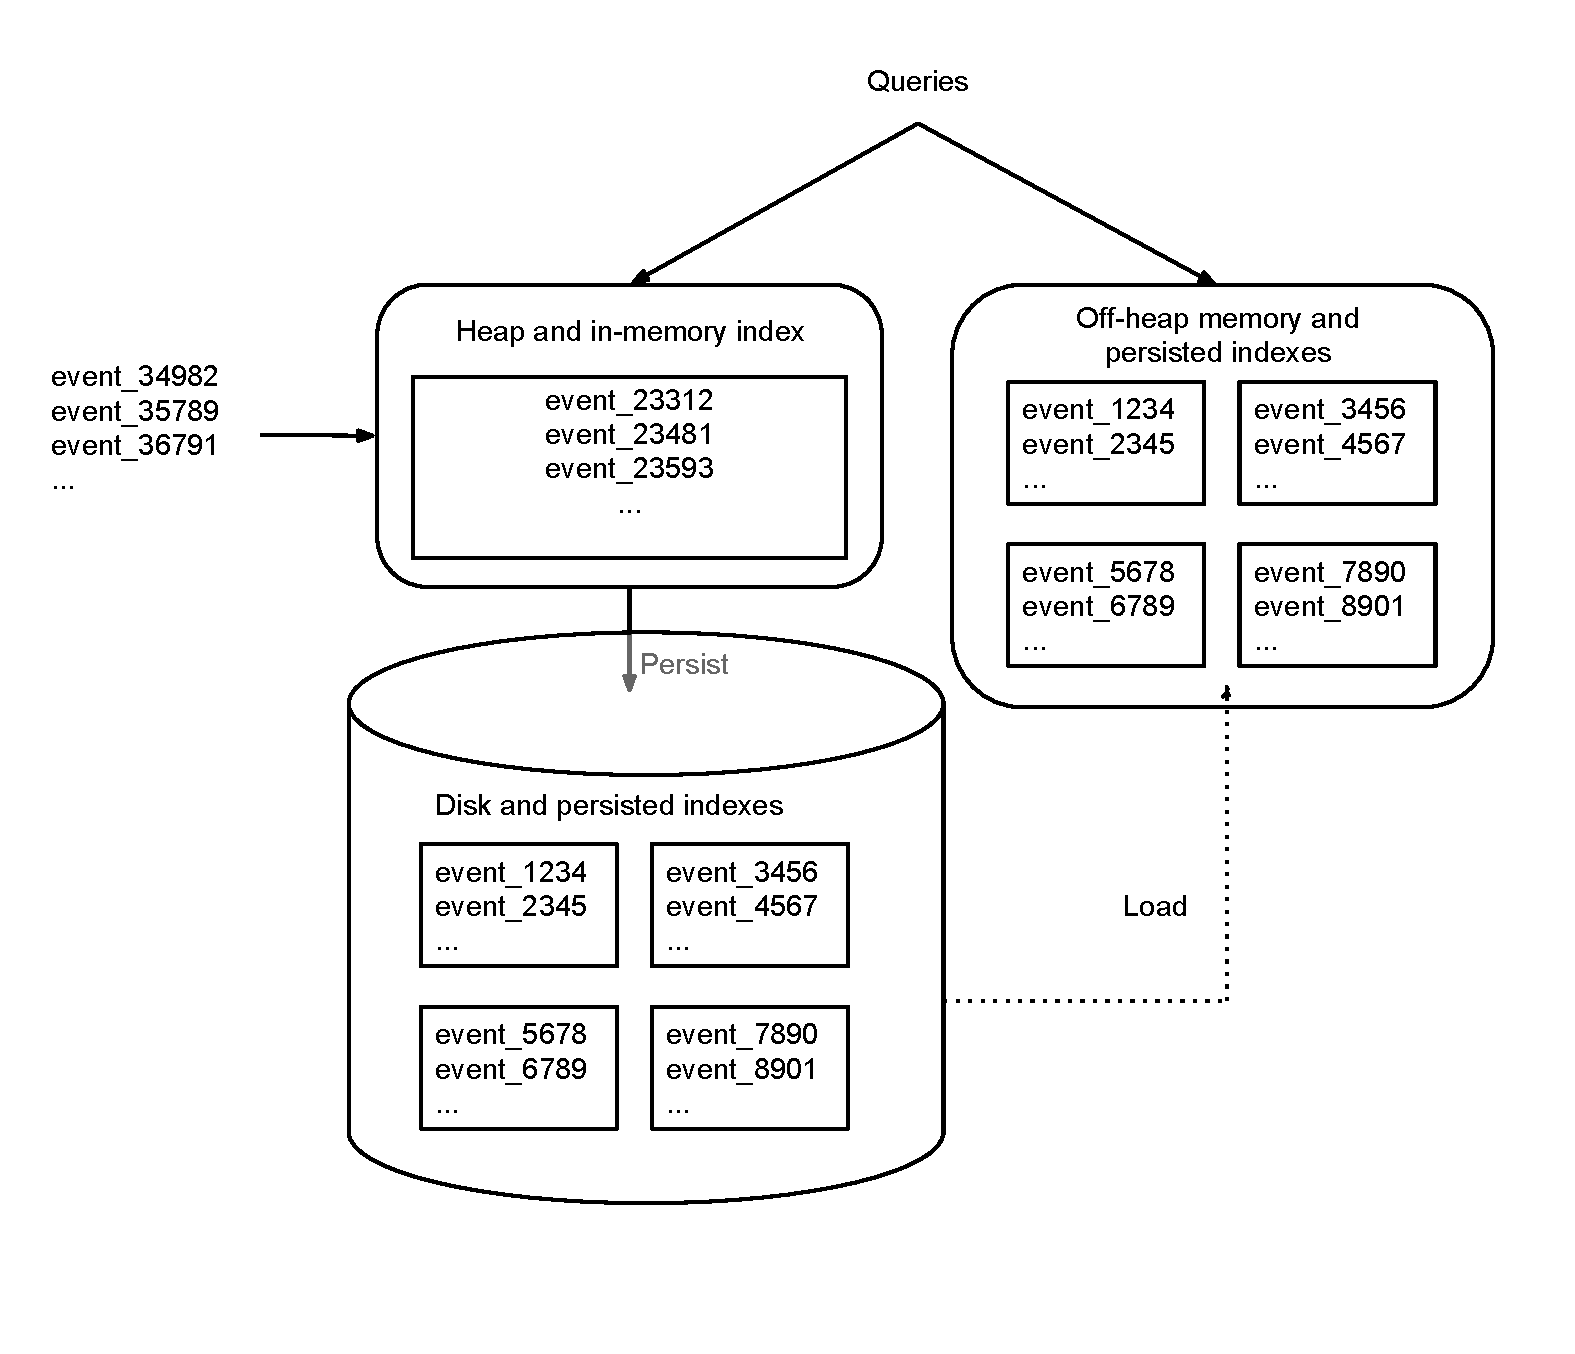
\includegraphics[width = 2.6in]{realtime_flow}
\caption{Real-time nodes buffer events to an in-memory index, which is
regularly persisted to disk. On a periodic basis, persisted indexes are then merged
together before getting handed off.
Queries will hit both the in-memory and persisted indexes.
}
\label{fig:realtime_flow}
\end{figure}

Real-time nodes employ a log structured merge tree\cite{o1996log} for recently
ingested data. Incoming events are first stored in an in-memory buffer. The
in-memory buffer is directly queryable and Druid behaves as a row store for
queries on events that exist in this JVM heap-based store. The in-memory buffer
is heavily write optimized, and given that Druid is really designed for heavy
concurrent reads, events do not remain in the in-memory buffer for very long.
To avoid heap overflow problems and to improve read latency, real-time nodes
persist their in-memory indexes to disk either periodically or after some
maximum row limit is reached. This persist process converts data stored in the
in-memory buffer to the column oriented segment storage format described in
Section \ref{sec:segments}.  Persisted segments are memory mapped and loaded
into off-heap memory such that they can still be queried. This is illustrated
in Figure~\ref{fig:realtime_timeline}. Data is continuously queryable during
the persist process.

Real-time ingestion in Druid is self-throttling. If a significant spike occurs
in the number of events transferred from the upstream event producer, there are
a few safety mechanisms built in. Recall that events are first stored in an
in-memory buffer and persists can occur when a maximum configurable row limit
is reached. Spikes in event volume should cause persists to occur more often
and not overflow the in-memory buffer. However, the process of building a
segment does require time and resources. If too many concurrent persists occur,
and if events are added to the in-memory buffer faster than they can be removed
through the persist process, problems can still arise. Druid sets a limit on
the maximum number of persists that can occur at a time, and if this limit is
reached, Druid will begin to throttle event ingestion. In this case, the onus
is on the upstream consumer to be resilient in the face of increasing backlog.

Real-time nodes store recent data for a configurable period of time, typically
an hour. This period is referred to as the segment granularity period. The
nodes employ a sliding window to accept and reject events and use the
wall-clock time as the basis of the window. Events within a configurable limit
before or after the node’s wall-clock time are accepted, and events outside
this window are dropped. This period is referred to as the window period and
typical window periods are 10 minutes in length. The window period is
illustrated in Figure []. At the end of the segment granularity period plus the
window period, a real-time node will hand off the data it has collected during
the segment granularity period. 

For further clarification, consider Figure~\ref{fig:realtime_timeline}.
Figure~\ref{fig:realtime_timeline} illustrates the operations of a real-time
node. The node starts at 13:37 and, with a 10 minute window period, will only
accept events for a window between 13:17 and 13:47.  When events are ingested,
the node announces that it is serving a segment of data for an interval from
13:00 to 14:00. Every 10 minutes (the persist period is configurable), the node
will flush and persist its in-memory buffer to disk.  Near the end of the hour,
the node will likely see events for 14:00 to 15:00.  When this occurs, the node
prepares to serve data for the next hour and creates a new in-memory buffer.
The node then announces that it is also serving a segment from 14:00 to 15:00.
The node does not immediately merge persisted indexes from 13:00 to 14:00,
instead it waits for a configurable window period for straggling events from
13:00 to 14:00 to arrive. This window period minimizes the risk of data loss
from delays in event delivery. At the end of the window period, the node merges
all persisted indexes from 13:00 to 14:00 into a single immutable segment and
hands the segment off. Once this segment is loaded and queryable somewhere else
in the Druid cluster, the real-time node flushes all information about the data
it collected for 13:00 to 14:00 and unannounces it is serving this data.

\begin{figure*}
\centering

\includegraphics[width = 4.5in]{realtime_timeline}
\caption{The node starts, ingests data, persists, and periodically hands data
off. This process repeats indefinitely. The time periods between different
real-time node operations are configurable.}
\label{fig:realtime_timeline}
\end{figure*}

The use of the window period means that events that are substantially delayed
will be dropped. In practice, we see that these occurrences are rare, but they
do occur. Druid’s real-time logic does not guarantee exactly once processing
and is instead best effort. The lack of exactly once processing in Druid is one
of the motivations for requiring batch fix up in the RADStack.

\subsection{Hand off}
Real-time nodes are designed to deal with a small window of recent data and
need periodically hand off segments they’ve built. The hand-off process first
involves a compaction step. The compaction process finds all the segments that
were created for a specific interval of time (for example, all the segments
that were created by intermediate persists over the period of an hour). These
segments are merged together to form a final immutable segment for handoff. 

Handoff occurs in a few steps. First, the finalized segment is uploaded to a
permanent backup storage, typically a distributed file system such as S3 [] or
HDFS [], which Druid refers to as “deep storage”. Next, an entry is created in
the metadata store (typically a RDBMS such as MySQL) to indicate that a new
segment has been created. This entry in the metadata store will eventually
cause other nodes in the Druid cluster to download and serve the segment. The
real-time node continues to serve the segment until it notices that the segment
is available on Druid historical nodes, which are nodes that are dedicated to
serving historical data. At this point, the segment is dropped and unannounced
from the real-time node. The entire handoff process is fluid; data remains
continuously queryable throughout the entire handoff process. Segments created
by real-time processing are versioned by the start of the segment granularity
interval.

\subsection{Batch Data Ingestion}
The core component used by real-time ingestion is an index that can be
incrementally populated and finalized to create an immutable segment. This core
component is shared across both real-time and batch ingestion. Druid has built
in support for creating segments by leveraging Hadoop and running MapReduce
jobs to partition data for segments.  Events can be “streamed” directly from
static files.

Similar to the real-time ingestion logic, segments created through batch
ingestion are directly uploaded to deep storage. Druid’s Hadoop-based batch
indexer will also create an entry in the metadata storage once all segments
have been created. The version of the segments created by batch ingestion are
based on the time the batch processing job starts at.

\subsection{Unifying Views}
When new entries are created in the metadata storage, they will eventually be
noticed by Druid coordinator nodes. Druid coordinator nodes poll the metadata
storage for what segments should be loaded on Druid historical nodes, and
compare the result with what is actually loaded on those nodes. Coordinator
nodes will tell historical nodes to load new segments, drop outdated segments,
and move segments across nodes.

Druid historical nodes are very simple in operation. They know how to load,
drop, and respond to queries that scan segments. Historical nodes typically
store all the data that is older than an hour (recent data lives on the
real-time node). The real-time handoff process requires that a historical must
load first load and begin serving queries for a segment before that segment can
be dropped from the real-time node. Since segments are immutable, the same copy
of a segment can exist on multiple historical nodes and real-time nodes. Most
nodes in typical production Druid clusters are historical nodes.

To consolidate results from historical and real-time nodes, Druid has a set of
broker nodes which act as the endpoint that clients query. Broker nodes
function as query routers to historical and real-time nodes. Broker nodes
understand the metadata published in Zookeeper about what segments are
queryable and where those segments are located. Broker nodes route incoming
queries such that the queries hit the right historical or real-time nodes.
Broker nodes also merge partial results from historical and real-time nodes
before returning a final consolidated result to the caller.

Broker nodes maintain a segment timeline containing information about what
segments exist in the cluster and the version of those segments. Druid uses
multi-version concuncurrency control to manage how data is extracted from
segments. Segments with higher version identifiers have precedence over
segments with lower version identifiers. If two segments exactly overlap for an
interval, Druid only considers the data from the segment with the higher
version interval.

Segments are inserted into the timeline as they are announced. The timeline
sorts the segment based on their data interval in a data structure similar to
an interval tree. Lookups in the timeline will return all segments with
intervals that overlap the lookup interval, along with interval ranges for
which the data in a segment is valid. This is illustrated in Figure [].

Brokers extract the interval of a query and use it for lookups into the
timeline. The result of the timeline is used to remap the original query into a
set of specific queries for the actual historical and real-time nodes that hold
the pertinent query data. This process is illustrated in Figure[]. The results
from the historical and real-time nodes are finally merged by the broker, which
returns the final result to the caller.

The coordinator node also builds a segment timeline for segments in the
cluster. If a segment is completely overshadowed by one or more segments, it
will be flagged in this timeline. When the coordinator notices overshadowed
segments, it tells historical nodes to drop these segments from the cluster.

\subsection{Supported Queries}
Druid has its own query language and accepts queries as POST requests. Broker,
historical, and real-time nodes all share the same query API. 

The body of the POST request is a JSON object containing key/value pairs
specifying various query parameters. A typical query will contain the data
source name, the granularity of the result data, time range of interest, the
type of request, and the metrics to aggregate over. The result will also be a
JSON object containing the aggregated metrics over the time period. 

Most query types will also support a filter set. A filter set is a Boolean
expression of dimension name and value pairs. Any number and combination of
dimensions and values may be specified. When a filter set is provided, only the
subset of the data that pertains to the filter set will be scanned. The ability
to handle complex nested filter sets is what enables Druid to drill into data
at any depth. 

The exact query syntax depends on the query type and the information requested.
A sample count query over a week of data is as follows: 

{\scriptsize\begin{verbatim}
{
  "queryType": "timeseries",
  "dataSource": “ads",
  "intervals": "2013-01-01\/2013-01-08",
  "filter": {
    "type": "selector",
    "dimension": "publisher",
    "value": "google.com"
  },
  "granularity": "day",
  "aggregations": [
    {
      "type": "count",
      "name": "rows"
    }
  ]
}
\end{verbatim}}

The query shown above will return a count of the number of rows in the “ads”
data source from 2013-01-01 to 2013-01-08, filtered for only those rows where
the value of the “publisher” dimension is equal to “google.com”. The results
will be bucketed by day and will be a JSON array of the following form: 

{\scriptsize\begin{verbatim}
[
  {
    "timestamp": "2012-01-01T00:00:00.000Z",
    "result": {
      "rows": 393298
    }
  },
  {
    "timestamp": "2012-01-02T00:00:00.000Z",
    "result": {
      "rows": 382932
    }
  },
  ...
  {
    "timestamp": "2012-01-07T00:00:00.000Z",
    "result": {
      "rows": 1337
    }
  }
]
\end{verbatim}}

Druid supports many types of aggregations including sums on floating-point and
integer types, minimums, maximums, and complex aggregations such as cardinality
estimation and approximate quantile estimation. The results of aggregations can
be combined in mathematical expressions to form other aggregations. It is
beyond the scope of this paper to fully describe the query API but more
information can be found
online\footnote{\href{http://druid.io/docs/latest/Querying.html}{http://druid.io/docs/latest/Querying.html}}. 

As of this writing, a join query for Druid is not yet implemented. This has
been a function of engineering resource allocation and use case decisions more
than a decision driven by technical merit. Indeed, Druid’s storage format would
allow for the implementation of joins (there is no loss of fidelity for columns
included as dimensions) and the implementation of them has been a conversation
that we have every few months. To date, we have made the choice that the
implementation cost is not worth the investment for our organization. The
reasons for this decision are generally two-fold. 

1. Scaling join queries has been, in our professional experience, a constant
bottleneck of working with distributed databases. 

2. The incremental gains in functionality are perceived to be of less value
than the anticipated problems with managing highly concurrent, join-heavy
workloads. 

A join query is essentially the merging of two or more streams of data based on
a shared set of keys. The primary high-level strategies for join queries we are
aware of are a hash-based strategy or a sorted-merge strategy. The hash-based
strategy requires that all but one data set be available as something that
looks like a hash table, a lookup operation is then performed on this hash
table for every row in the “primary” stream. The sorted-merge strategy assumes
that each stream is sorted by the join key and thus allows for the incremental
joining of the streams. Each of these strategies, however, requires the
materialization of some number of the streams either in sorted order or in a
hash table form.

When all sides of the join are significantly large tables (> 1 billion
records), materializing the pre-join streams requires complex distributed
memory management. The complexity of the memory management is only amplified by
the fact that we are targeting highly concurrent, multi-tenant workloads. For
these reasons, we’ve elected to do joins at the processing layer for the time
being.

\section{The Processing Layer}
\label{sec:processing}
Although Druid can ingest events that are streamed in one at a time, data must
be denormalized before it is ingested in Druid, as Druid cannot yet support
join queries. Furthermore, real world data must often be transformed before it
is usable by an application.

\subsection{Stream Processing}
\label{sec:streamprocessing}
Stream processors provide infrastructure to develop processing logic for
unbounded sequences of tuples. We will focus our discussions on Apache Samza as
our stream processor, although other technologies are viable alternatives.
Samza provides an API to write jobs that run over a sequence of tuples and
perform operations over those tuples in a user-defined way. The input to each
job is provided by Kafka, which can also act as a sink for the output of the
job. Samza jobs are executed in a resource management and task execution
framework such as YARN []. It is beyond the scope of this paper to go into the
full details of Kafka/YARN/Samza interactions, but more information is
available in other literature []. We will instead focus on how we leverage this
framework for processing data for analytic use cases.

On top of Samza infrastructure, we introduce the idea of a “pipeline”, which is
a grouping for a series of related processing jobs, sorted in some logical
order. The output of one job may act as the input for the next job. Some of our
jobs involve operations include renaming data, inserting default values for
nulls and empty strings, and filtering data. One pipeline maps logically to one
data source in Druid.

Given that Druid does not support joins in queries, we require supporting joins
at the data processing level. Our approach to do streaming joins is to leverage
a key/value store such as Redis[] and buffer events in memory for a given
period of time. If an event arrives in the system with a join key that exists
in the key/value store, the join occurs and the joined event is transmitted
further down the pipeline. If events are substantially delayed and do not
arrive in the allocated window period, the original event is dropped. This
means that our stream processing layer is not guaranteed to deliver 100%
accurate results. Furthermore, Samza does not offer exactly-once processing
semantics. Problems in network connectivity or node failure can lead to
duplicated events. For this reason, we run a separate batch pipeline that will
generate an accurate copy of the ingested data.

The final job in our processing pipeline is to deliver data to Druid. For high
availability, processed events from Samza are transmitted concurrently to two
real-time nodes. Both nodes receive the same copy of data, and one node
effectively acts as a replica. The Druid broker does not distinguish between
the two copies of data, and queries will go to either node. When handoff
occurs, both real-time nodes race to hand off the segments they’ve created. The
segment that is pushed into deep storage first will be the one that is used for
historical querying, and once that segment is loaded on the historical nodes,
both real-time nodes will drop their versions of the same segment.

\subsection{Batch Processing}
Our batch processing pipeline is composed of two stages. The first stage
mirrors our streaming processing pipeline in that it transforms data and joins
relevant events in preparation for the is data to be loaded into Druid. This is
done via a MapReduce job, similar to the setup described in []. The second
stage of batch processing is responsible for directly creating immutable Druid
segments. We can run a second MapReduce\cite{dean2008mapreduce} job that feeds reads our processed
data from the first stage and loads this data into Druid’s built in ingestion
logic. The ingestion code for both streaming and batch ingestion in Druid is
shared between the two modes of ingestion. The batch processing logic uploads
these segments to deep storage, and writes a new entry in the metadata store to
indicate that new segments are available. To Druid, there is no difference
between segments generated by the real-time logic with those generated by batch
processing, and Druid will proceed to load the batch generated segments.

Our ingestion model is hopefully more clear at this point. We use the streaming
data pipeline described in Section\ref{sec:streamprocessing} to deliver
immediate insights on events as they are occurring, and the batch data pipeline
described in this section to provide the accurate copy of the data. The batch
process typically runs much less frequently than the real-time process, and may
run many hours or even days after raw events have been delivered. The wait is
necessary for severely delayed events, and to ensure that the raw data is
indeed complete. 

Segments generated by the batch process are versioned by the start time of the
process. Hence, segments created by batch processing will have a version
identifier that is greater than segments created by real-time processing. When
these batch created segments are loaded in the cluster, they atomically replace
segments created by real-time processing for their processed interval. Hence,
soon after batch processing completes, Druid switches to querying for the
accurate copy of the data.

\subsection{Starfire}
To avoid writing the same processing logic on both Hadoop and Samza, we created
a library called Starfire to help generate workflows on both batch and stream
processing frameworks. Starfire has a streaming model of computation at its
heart, even when running in batch mode. It is designed to never need to load up
all your data at once, in any mode of operation, but it offers operators that
do need to work across multiple data points, like “groupBy” and “join”. Since
these operators cannot run across the entire data set, Starfire runs them using
windows.

Starfire programs ask for a particular window size (measured in time, like 15
minutes or two hours) that particular drivers must provide. The Hadoop driver
provides a window size by loading up data surrounding the data that you are
actually interested in. The Samza driver does it by buffering data in a
key/value store for a period of time. Starfire supports using different window
sizes from driver to driver, which can be useful if you are running a
combination batch/real-time architecture. We hope to explore Starfire more in
future literature.

\section{The Delivery Layer}
\label{sec:delivery}
In our stack, events are delivered over HTTP to Kafka. Events are transmitted
via POST requests to a receiver that acts as a front for a Kafka producer.
Kafka is a distributed messaging system with a publish and subscribe model. At
a high level, Kafka maintains events or messages in categories called topics. A
distributed Kafka cluster consists of numerous brokers, which store messages in
a replicated commit log. Kafka consumers subscribe to topics and process feeds
of published messages. 

Kafka provides isolation of functionality in terms with producers of data and
consumers of data. The publish/subscribe model works well for our use case as
multiple consumers can subscribe to the same topic and process the same set of
events. We have two primary Kafka consumers. The first is a Samza job that
reads messages from Kafka for stream processing as described in Section
\ref{sec:streamprocessing}. The second consumer read messages from Kafka and
stores them in a distributed file system, similar to Camus []. This file system
is the same as the one used for Druid’s deep storage, and also acts as a backup
for raw events. Topics in Kafka map directly to pipelines in Samza, and
pipelines in Samza map directly to data sources in Druid. The purpose of
storing raw events in deep storage is so that we can run batch processing jobs
over them at any given time. For example, our stream processing layer may
choose to not include certain columns when it first processes a few pipeline.
If clients demand these columns be included in the future, we can reprocess the
raw data to generate new Druid segments. 

Kafka is the single point of delivery for events entering our system, and must
have the highest availability. We replicate our Kafka producers across multiple
datacenters. In the event that Kafka brokers and consumers become unresponsive,
as long as our HTTP endpoints are still available, we can buffer events on the
producer side while recovering the system. Similarity, if our processing and
serving layers completely fail, we can recover by replaying events from Kafka.

\section{Performance}
\label{sec:performance}
Druid runs in production at several organizations, and to briefly demonstrate
its performance, we have chosen to share some real world numbers for the main
production cluster running at Metamarkets in early 2015. For comparison with
other databases we also include results from synthetic workloads on TPC-H data.

\subsection{Query Performance in Production}
Druid query performance can vary signficantly depending on the query being
issued. For example, sorting the values of a high cardinality dimension based
on a given metric is much more expensive than a simple count over a time range.
To showcase the average query latencies in a production Druid cluster, we
selected 8 of our most queried data sources, described in
Table~\ref{tab:datasources}.

Approximately 30\% of queries are standard aggregates involving different types
of metrics and filters, 60\% of queries are ordered group bys over one or more
dimensions with aggregates, and 10\% of queries are search queries and metadata
retrieval queries. The number of columns scanned in aggregate queries roughly
follows an exponential distribution. Queries involving a single column are very
frequent, and queries involving all columns are very rare.

\begin{table}
  \centering
  \scriptsize\begin{tabular}{| l | l | l |}
    \hline
    \textbf{Data Source} & \textbf{Dimensions} & \textbf{Metrics} \\ \hline
    \texttt{a} & 25 & 21 \\ \hline
    \texttt{b} & 30 & 26 \\ \hline
    \texttt{c} & 71 & 35 \\ \hline
    \texttt{d} & 60 & 19 \\ \hline
    \texttt{e} & 29 & 8 \\ \hline
    \texttt{f} & 30 & 16 \\ \hline
    \texttt{g} & 26 & 18 \\ \hline
    \texttt{h} & 78 & 14 \\ \hline
  \end{tabular}
  \normalsize
  \caption{Characteristics of production data sources.}
  \label{tab:datasources}
\end{table}

\begin{itemize}[leftmargin=*,beginpenalty=5000,topsep=0pt]
\item The results are from a ``hot" tier in our production cluster. There were
approximately 50 data sources in the tier and several hundred users issuing
queries.

\item There was approximately 10.5TB of RAM available in the ``hot" tier and
approximately 10TB of segments loaded. Collectively,
there are about 50 billion Druid rows in this tier. Results for
every data source are not shown.

\item The hot tier uses Intel\textsuperscript{\textregistered} Xeon\textsuperscript{\textregistered} E5-2670 processors and consists of 1302 processing
threads and 672 total cores (hyperthreaded).

\item A memory-mapped storage engine was used (the machine was configured to
    memory map the data instead of loading it into the Java heap.)
\end{itemize}

Query latencies are shown in Figure~\ref{fig:query_latency} and the queries per
minute are shown in Figure~\ref{fig:queries_per_min}. Across all the various
data sources, average query latency is approximately 550 milliseconds, with
90\% of queries returning in less than 1 second, 95\% in under 2 seconds, and
99\% of queries returning in less than 10 seconds. Occasionally we observe
spikes in latency, as observed on February 19, where network issues on
the Memcached instances were compounded by very high query load on one of our
largest data sources.

\begin{figure}
\centering
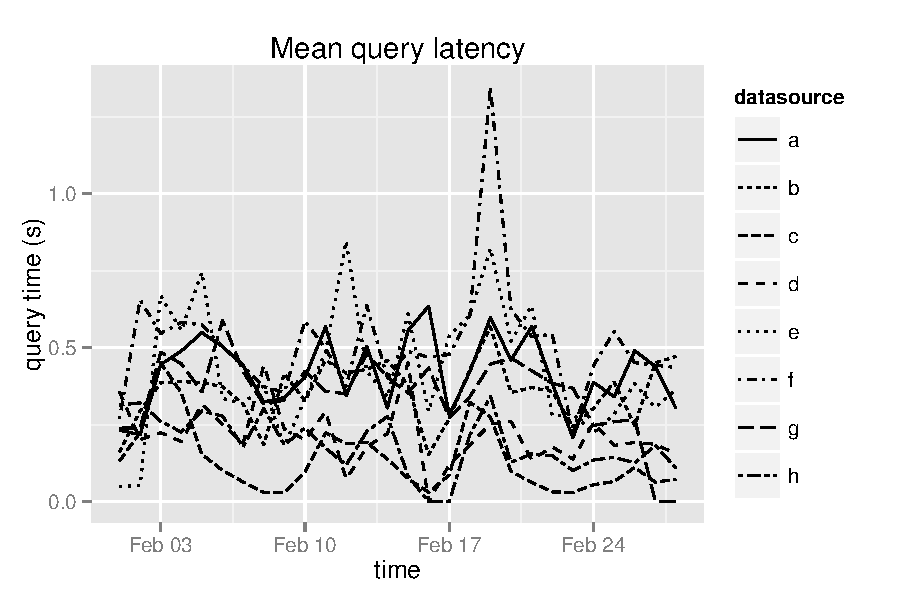
\includegraphics[width = 2.3in]{avg_query_latency}
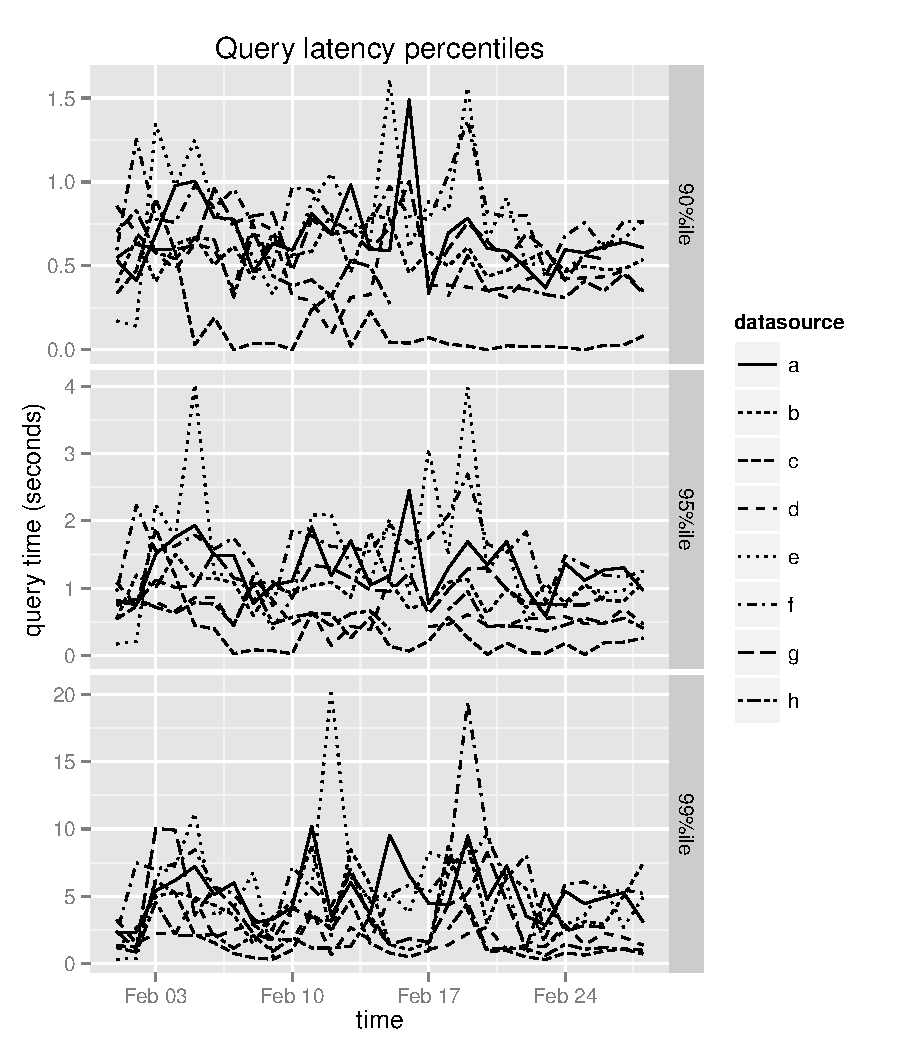
\includegraphics[width = 2.3in]{query_percentiles}
\caption{Query latencies of production data sources.}
\label{fig:query_latency}
\end{figure}

\begin{figure}
\centering
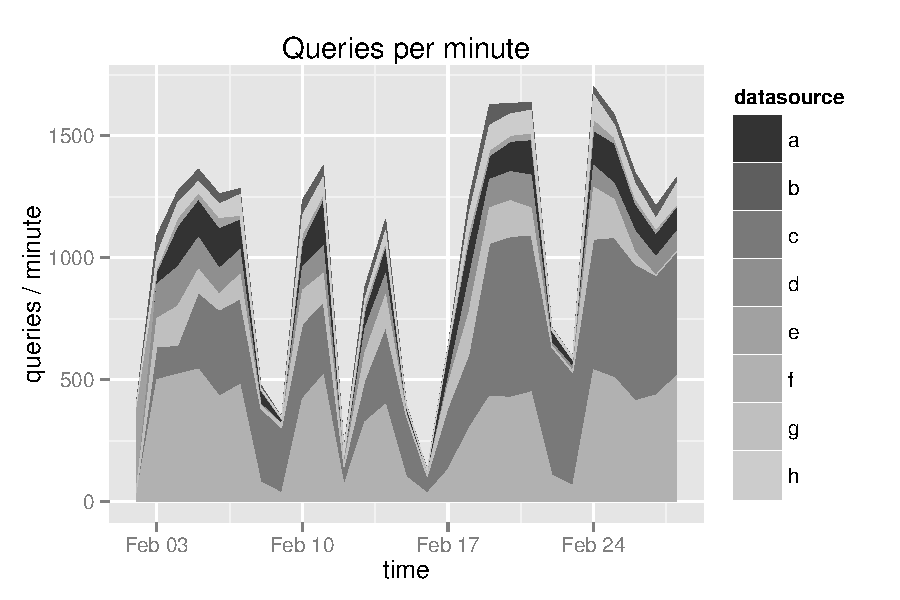
\includegraphics[width = 2.8in]{queries_per_min}
\caption{Queries per minute of production data sources.}
\label{fig:queries_per_min}
\end{figure}

\subsection{Query Benchmarks on TPC-H Data}
We also present Druid benchmarks on TPC-H data.  Most TPC-H queries do not
directly apply to Druid, so we selected queries more typical of Druid's
workload to demonstrate query performance. 

Our Druid setup used Amazon EC2 \texttt{m3.2xlarge} instance types
(Intel\textsuperscript{\textregistered} Xeon\textsuperscript{\textregistered}
E5-2680 v2 @ 2.80GHz) for historical nodes and \texttt{c3.2xlarge} instances
(Intel\textsuperscript{\textregistered} Xeon\textsuperscript{\textregistered}
E5-2670 v2 @ 2.50GHz) for broker nodes. Our MySQL setup was an Amazon RDS
instance that ran on the same \texttt{m3.2xlarge} instance type.

The results for the 1 GB TPC-H data set are shown in Figure~\ref{fig:tpch_1gb}
and the results of the 100 GB data set are shown in
Figure~\ref{fig:tpch_100gb}. We benchmarked Druid's scan rate at 53,539,211
rows/second/core for \texttt{select count(*)} equivalent query over a given
time interval and 36,246,530 rows/second/core for a \texttt{select sum(float)}
type query.

\begin{figure}
\centering
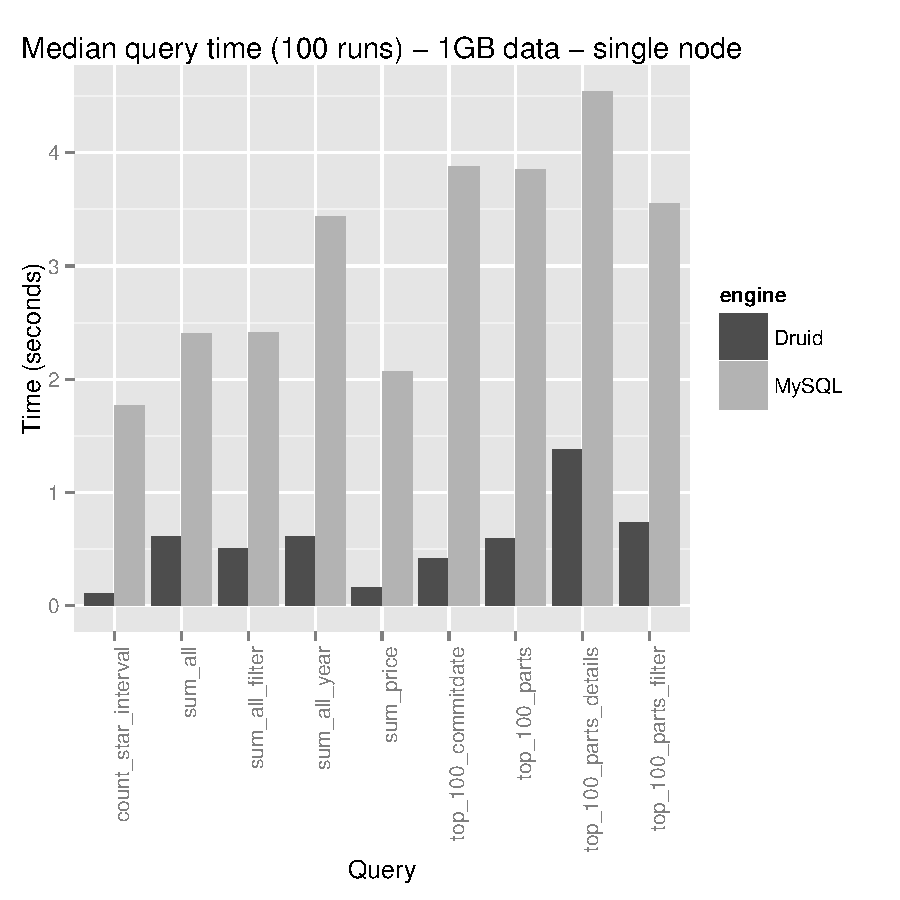
\includegraphics[width = 2.3in]{tpch_1gb}
\caption{Druid benchmarks -- 1GB TPC-H data.}
\label{fig:tpch_1gb}
\end{figure}

\begin{figure}
\centering
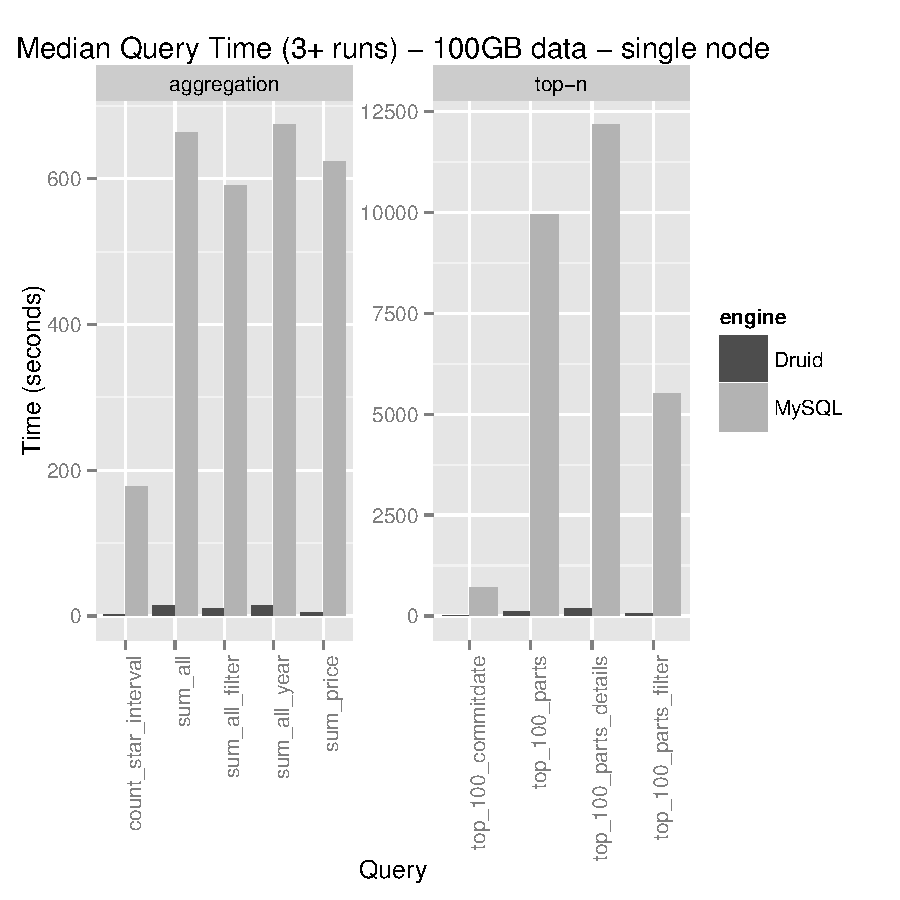
\includegraphics[width = 2.3in]{tpch_100gb}
\caption{Druid benchmarks -- 100GB TPC-H data.}
\label{fig:tpch_100gb}
\end{figure}

Finally, we present our results of scaling Druid to meet increasing data
volumes with the TPC-H 100 GB data set. We observe that when we
increased the number of cores from 8 to 48, not all types of queries
achieve linear scaling, but the simpler aggregation queries do,
as shown in Figure~\ref{fig:tpch_scaling}.

he increase in speed of a parallel computing system is often limited by the
time needed for the sequential operations of the system. In this case, queries
requiring a substantial amount of work at the broker level do not parallelize as
well.

\begin{figure}
\centering
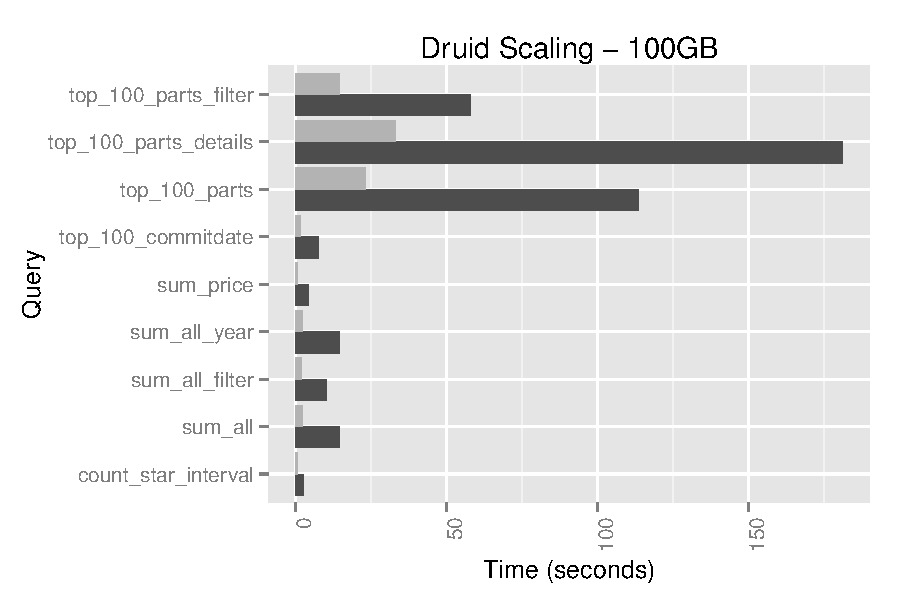
\includegraphics[width = 2.3in]{tpch_scaling}
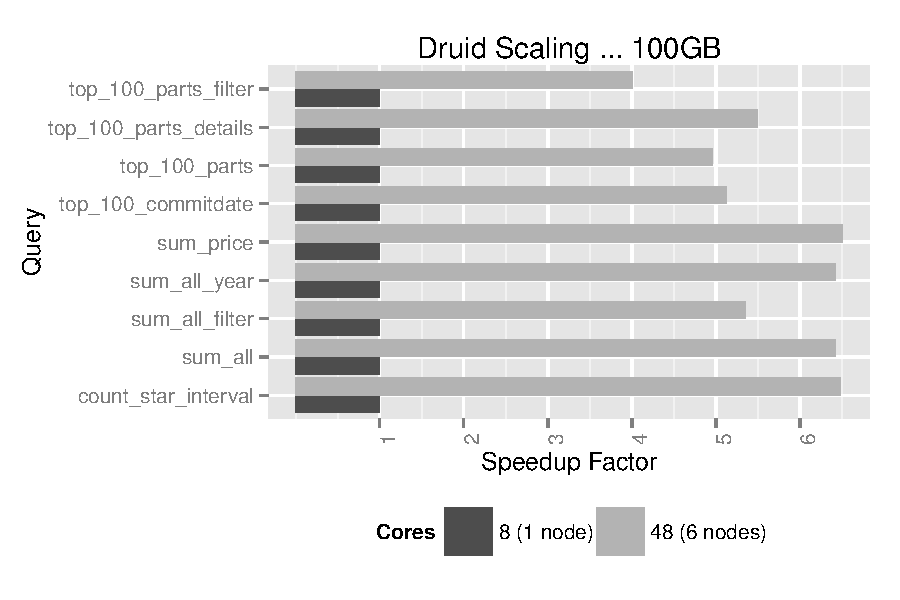
\includegraphics[width = 2.3in]{tpch_scaling_factor}
\caption{Druid scaling benchmarks -- 100GB TPC-H data.}
\label{fig:tpch_scaling}
\end{figure}

\subsection{Data Ingestion Performance}
To showcase Druid's data ingestion latency, we selected several production
datasources of varying dimensions, metrics, and event volumes. Our production
ingestion setup consists of 6 nodes, totalling 360GB of RAM and 96 cores (12 x
Intel\textsuperscript\textregistered Xeon\textsuperscript\textregistered
E5-2670).

Note that in this setup, several other data sources were being ingested and
many other Druid related ingestion tasks were running concurrently on the
machines.

Druid's data ingestion latency is heavily dependent on the complexity of the
data set being ingested. The data complexity is determined by the number of
dimensions in each event, the number of metrics in each event, and the types of
aggregations we want to perform on those metrics. With the most basic data set
(one that only has a timestamp column), our setup can ingest data at a rate of
800,000 events/second/core, which is really just a measurement of how fast we
can deserialize events. Real world data sets are never this simple.
Table~\ref{tab:ingest_datasources} shows a selection of data sources and their
characteristics.

\section{Production Experiences}
\label{sec:experiences}

\subsection{Experiences with Druid}
\subsubsection{Query Patterns}
Druid is used for exploratory analytics and reporting, which are two very
distinct use cases. Exploratory analytic workflows uncover discoveries by
progressively narrowing down a view of data until an interesting insight is
made. Users tend to explore short intervals of recent data. In the reporting
use case, users query for much longer data intervals, and the volume of queries
is generally much less. The insights that users are looking for are often
pre-determined. 

\subsubsection{Multitenancy}
Expensive concurrent queries can be problematic in a multitenant environment.
Queries for large data sources may end up hitting every historical node in a
cluster and consume all cluster resources. Smaller, cheaper queries may be
blocked from executing in such cases. We introduced query prioritization to
address these issues. Each historical node is able to prioritize which segments
it needs to scan. Proper query planning is critical for production workloads.
Thankfully, queries for a significant amount of data tend to be for reporting
use cases and can be de-prioritized. Users do not expect the same level of
interactivity in this use case as they do when they are exploring data. 

\subsubsection{Node Failures}
Single node failures are common in distributed environments, but many nodes
failing at once are not. If historical nodes completely fail and do not
recover, their segments need to be reassigned, which means we need excess
cluster capacity to load this data. The amount of additional capacity to have
at any time contributes to the cost of running a cluster. From our experiences,
it is extremely rare to see more than 2 nodes completely fail at once and
hence, we leave enough capacity in our cluster to completely reassign the data
from 2 historical nodes. 

\subsection{Experiences with Ingestion}
\subsubsection{Multitenancy}
Before moving our streaming pipeline to Samza, we experimented with other
stream processors. One of the biggest pains we felt was multi-tenancy. Multiple
pipelines may contend for resources, and it is often unclear how various jobs
impact one another when running in the same environment. Given that each of our
pipelines is composed of different tasks, Samza was able to provide per task
resource isolation, which was far easier to manage than per application
resource isolation.

\subsubsection{Autoscaling}
Autoscaling our cluster to adjust for changes in load has remained a difficult
problem. Production load is not constant, and different peaks can occur at
vastly different times during a day. We’ve elected to focus on the problem of
gradually increasing load, instead dealing with immediate spikes or dips in
load. As load increases, we add new resources but set a configurable limit on
how fast they can be added. We scale down our cluster very slowly, excess
capacity may remain for several hours before the system decides they are no
longer necessary.

\subsection{Operational Monitoring}
Proper monitoring is critical to run a large scale distributed cluster,
especially with many different technologies. Each Druid node is designed to
periodically emit a set of operational metrics. These metrics may include
system level data such as CPU usage, available memory, and disk capacity, JVM
statistics such as garbage collection time, and heap usage, or node specific
metrics such as segment scan time, cache hit rates, and data ingestion
latencies. Druid also emits per query metrics so we can examine why a
particular query may be slow. We’ve also added functionality to periodically
emit metrics from Samza, Kafka, and Hadoop. We emit metrics from our production
RADStack and load them into a dedicated metrics RADstack. The metrics cluster
is used to explore the performance and stability of the production cluster.
This dedicated metrics cluster has allowed us to find numerous production
problems, such as gradual query speed degradations, less than optimally tuned
hardware, and various other system bottlenecks. We also use a metrics cluster
to analyze what queries are made in production and what aspects of the data
users are most interested in.

\section{Related Work}
\label{sec:related}

\subsection{Hybrid Batch/Streaming Workflows}

\subsubsection{Summingbird}
Summingbird[] is a high-level dataflow language for streaming and batch
processing. Summingbird enables counters on top of streams, and processes data
for delivery to key/value stores. Summingbird can run on top of data processors
such as Storm[] and Hadoop. The RADStack also offers a language for writing
data processing jobs with Starfire. These jobs do not involve computation and
focus entirely on data processing. Starfire enables more complex operations
such as streaming joins. Moreover, the RADStack leaves all queries and
aggregations to the serving layer, letting each layer of the stack focus on
what it is best at.

\subsubsection{Spark Ecosystem}
Spark[] is a cluster computing framework optimized for iterative workflows.
Spark Streaming[] is a separate project that converts sequences of tuples into
immutable micro-batches. Each micro-batch can be processed using the underlying
Spark framework. Spark SQL is a query optimization layer that can sit on top of
Spark and issue SQL queries, along with Spark’s native analytic queries.
Druid’s approach to querying is quite different and Druid insteads builds
immutable indexed data structures optimized for low latency OLAP queries, and
does not leverage lineage[] in computations. The RADStack can theoretically be
composed of Spark and Spark Streaming for processing, Kafka for event delivery,
and Druid to serve queries.

\subsection{Druid and Other Data Stores}
Although Druid builds on many of the same principles as other distributed
columnar data stores\cite{fink2012distributed}, many of these data stores are
designed to be more generic key-value stores\cite{lakshman2010cassandra} and do
not support computation directly in the storage layer. There are also other
data stores designed for some of the same data warehousing issues that Druid is
meant to solve. These systems include in-memory databases such as SAP’s
HANA\cite{farber2012sap} and VoltDB\cite{voltdb2010voltdb}. These data stores
lack Druid’s low latency ingestion characteristics. Druid also has native
analytical features baked in, similar to ParAccel\cite{paraccel2013}, however,
Druid allows system wide rolling software updates with no downtime. 

Druid is similar to C-Store\cite{stonebraker2005c} and
LazyBase\cite{cipar2012lazybase} in that it has two subsystems, a
read-optimized subsystem in the historical nodes and a write-optimized
subsystem in real-time nodes. Real-time nodes are designed to ingest a high
volume of append heavy data, and do not support data updates. Unlike the two
aforementioned systems, Druid is meant for OLAP transactions and not OLTP
transactions. Druid’s low latency data ingestion features share some
similarities with Trident/Storm\cite{marz2013storm} and Spark
Streaming\cite{zaharia2012discretized}, however, both systems are focused on
stream processing whereas Druid is focused on ingestion and aggregation. Stream
processors are great complements to Druid as a means of pre-processing the data
before the data enters Druid. 

There are a class of systems that specialize in queries on top of cluster
computing frameworks. Shark\cite{engle2012shark} is such a system for queries
on top of Spark, and Cloudera’s Impala\cite{cloudera2013} is another system
focused on optimizing query performance on top of HDFS. Druid historical nodes
download data locally and only work with native Druid indexes. We believe this
setup allows for faster query latencies. Druid leverages a unique combination
of algorithms in its architecture. Although we believe no other data store has
the same set of functionality as Druid, some of Druid’s optimization techniques
such as using inverted indices to perform fast filters are also used in other
data stores\cite{macnicol2004sybase}. 

\section{Conclusions and Future Work}
\label{sec:conclusions}
In this paper we presented the RADStack, a collection of complementary
technologies that can be used together to power interactive analytic
applications. The key pieces of the stack are Kafka, Samza, Hadoop, and Druid.
Druid is designed for exploratory analytics and is optimized for low latency
data exploration, aggregation, and ingestion, and is well suited for OLAP
workflows. Samza and Hadoop complement Druid and add data processing
functionality, and Kafka solves the event delivery problem. 

We believe that although our solution currently requires batch processing, in
later iterations of this work, that piece of the stack may not be necessary. As
open source technologies mature, the existing problems around exactly-once
processing will eventually be solved. The Druid, Samza and Kafka communities
are actively working on exactly once, lossless processing for their respective
systems, and in the near future, the same guarantees that the RADStack provides
right now will be available using only these technologies.

%\end{document}  % This is where a 'short' article might terminate

% ensure same length columns on last page (might need two sub-sequent latex runs)
\balance

%ACKNOWLEDGMENTS are optional
\section{Acknowledgments}
Druid, Samza, Kafka, and Hadoop could not have been built the assistance of
their respective communities. We want to thank everyone that contributes to
open source for their invaluable support.

% The following two commands are all you need in the
% initial runs of your .tex file to
% produce the bibliography for the citations in your paper.
\bibliographystyle{abbrv}
\bibliography{radstack}  % vldb_sample.bib is the name of the Bibliography in this case
% You must have a proper ".bib" file
%  and remember to run:
% latex bibtex latex latex
% to resolve all references

\end{document}
